\documentclass{Pretexto/bluereport}

\title{Manual de usuario}
\author{}
\date{}

\begin{document}

\begin{titlepage}
    \thispagestyle{empty}
    
    \pagecolor{white}
    
    % Ahora dibujamos las bandas laterales con \rule{}
    \begin{picture}(0,0)
        % Primera banda (amarilla, la más a la izquierda)
        \put(-94,-800){\textcolor{yellowdark}{\rule{3cm}{99.7cm}}} 
        % Segunda banda (verde)
        \put(-48,-800){\textcolor{yellowlight}{\rule{1.5cm}{99.7cm}}}
        % Tercera banda (azul)
        \put(-20,-800){\textcolor{primaryblue}{\rule{1cm}{99.7cm}}}
    \end{picture}
    
    % Contenido principal de la portada
    \begin{flushleft}
        \vspace*{1cm}

        % Ajusta este valor para mover todo hacia la derecha
        \hspace*{4.5cm}
        \begin{minipage}{13cm} % ancho de bloque de texto
            % Logo 

            
\includegraphics[width=6cm]{img/logo.png}


            \vspace{3cm} 
            
            % Títulos y texto
            {\fontsize{24}{28}\selectfont\color{primaryblue}
            \textbf{COTIZADOR LA LIGA}\par}

            \vspace{2cm}

            {\fontsize{36}{42}\selectfont\color{primaryblue}
            \textbf{Manual de Usuario}\par}
            
            \vspace{1cm}
            
            {\fontsize{16}{20}\selectfont\color{charcoal}
            Versión 1.0\par}
            
            \vfill 
            
            \rule{10cm}{1pt}
            
            \vspace{0.5cm}
            
            {\fontsize{16}{20}\selectfont\color{charcoal}
            Septiembre 2025\par}
        \end{minipage}
    \end{flushleft}
\end{titlepage}
\tableofcontents
\pagebreak

%%%%%%%%%%%%%%%%%%%%%%%%%%%%%%%%%%%%%%%%%%%%%%%%%%%%
\section{Introducción}

Breve descripción del software.

Propósito del manual.

A quién va dirigido (usuarios, administradores, etc.).

%%%%%%%%%%%%%%%%%%%%%%%%%%%%%%%%%%%%%%%%%%%%%%%%%%%%
\section{Requisitos del Sistema}

\subsection{Hardware y software necesarios.}


\subsection{Sistemas operativos compatibles.}

Se implementa un bucle iterativo que evalúa diferentes valores de k (de 2 a 10 clusters) utilizando cuatro métricas de validación. Para cada valor de k, se ajusta un modelo K-Means y se calculan todas las métricas de evaluación.

\begin{importante}[Configuración del Modelo]
Para garantizar la reproducibilidad de los resultados, se utiliza un estado aleatorio .
\end{importante}
-


%%%%%%%%%%%%%%%%%%%%%%%%%%%%%%%%%%%%%%%%%%%%%%%%%%%%
\section{Acceso}
\subsection{Cómo abrir la aplicaión}

Para abir la aplicacion, simplemente haga doble clic en el archivo ejecutable o utilice el acceso directo creado durante la instalación.
%%%%%%%%%%%%%%%%%%%%%%%%%%%%%%%%%%%%%%%%%%%%%%%%%%%%
\section{Interaz Principal y Funcionalidades}
\subsection{Explicación del menú de Gestión de Cotizaciones}

En el menu de getión de cotizaciones, se muestran todas las cotizaciones previamente realizadas, con opciones para editar, eliminar o generar el PDF de cada una.

\begin{figure}[H]
    \centering
    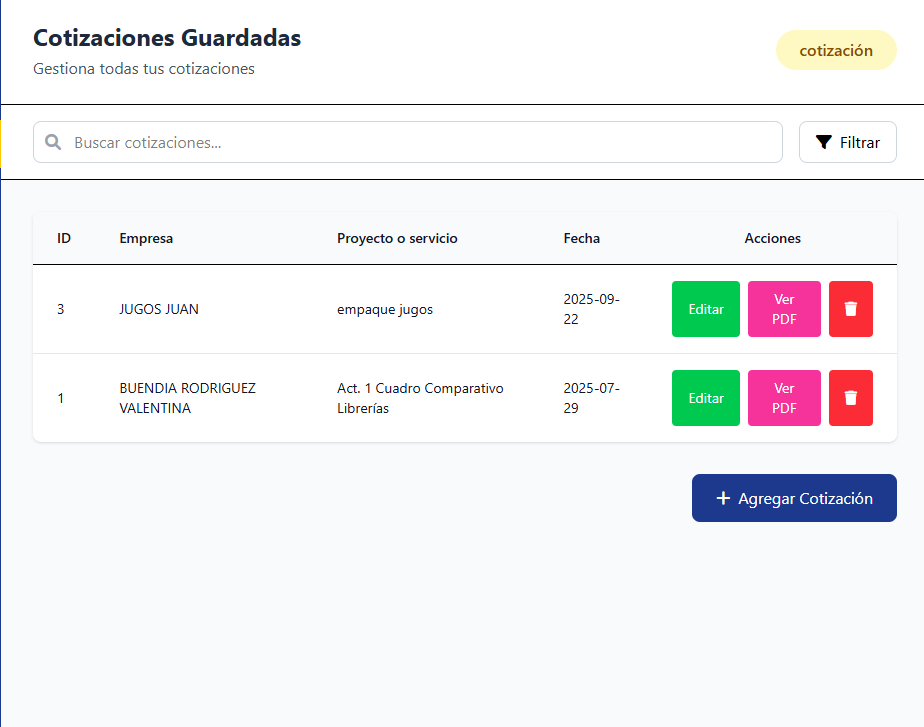
\includegraphics[width=0.8\textwidth]{Imagenes/gestion_cotizaciones.png}
    \caption{Menú de Gestión de Cotizaciones}
    \label{fig:gestion_cotizaciones}
\end{figure}

Ademas, se incluye un botón para agregar nuevas cotizaciones.

\begin{figure}[H]
    \centering
    
\includegraphics[width=0.8\textwidth]{Imagenes/agregar_cotizacion.png}
    \caption{Botón para Agregar Cotización}
    \label{fig:agregar_cotizacion}
\end{figure}

\subsection{Página para agregar cotizaciones}

En la pagina para agregar cotizaciones, se encuentran varios campos para ingresar los datos necesarios, como el nombre del cliente, la fecha, los productos o servicios a cotizar, y cualquier otro detalle relevante.
Ademas, se incluye un campo para importar datos desde un archivo Excel, para ello, se debe seleccionar el archivo deseado y la hoja correspondiente.

\begin{figure}[H]
    \centering
    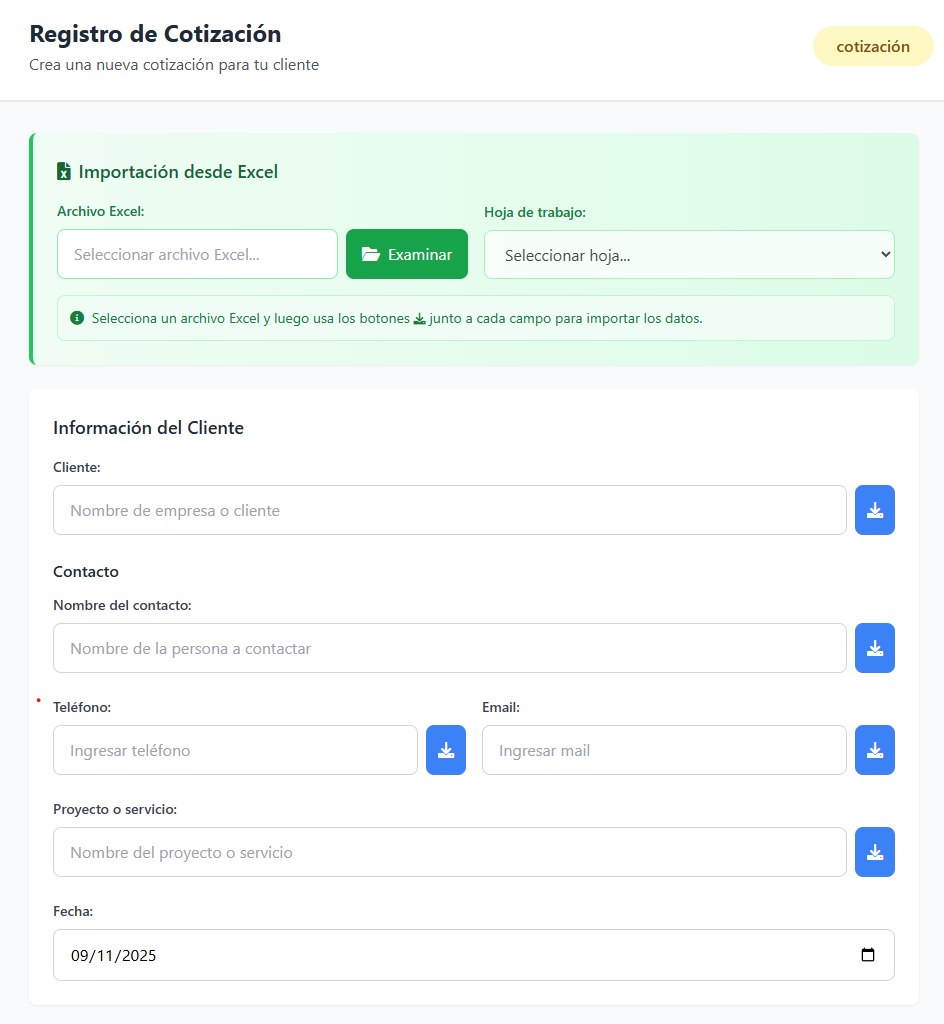
\includegraphics[width=0.8\textwidth]{Imagenes/agregar_cotizacion_pagina.png}
    \caption{Página para Agregar Cotizaciones}
    \label{fig:agregar_cotizacion_pagina}
\end{figure}

Para cada campo, hay un boton, que permite al usuario ingresar la informacioón desde el archivo Excel seleccionado, abriendo una nueva ventana con la opcion de dar click sobre la informacion deseada.

\begin{figure}[H]
    \centering
    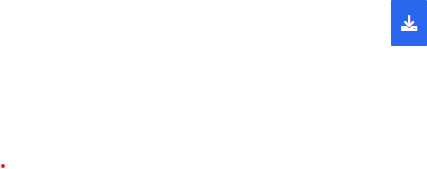
\includegraphics[width=0.8\textwidth]{Imagenes/boton_importacion.png}
    \caption{Boton para importar datos desde Excel}
    \label{fig:importar_datos}
\end{figure}

\begin{figure}[H]
    \centering
    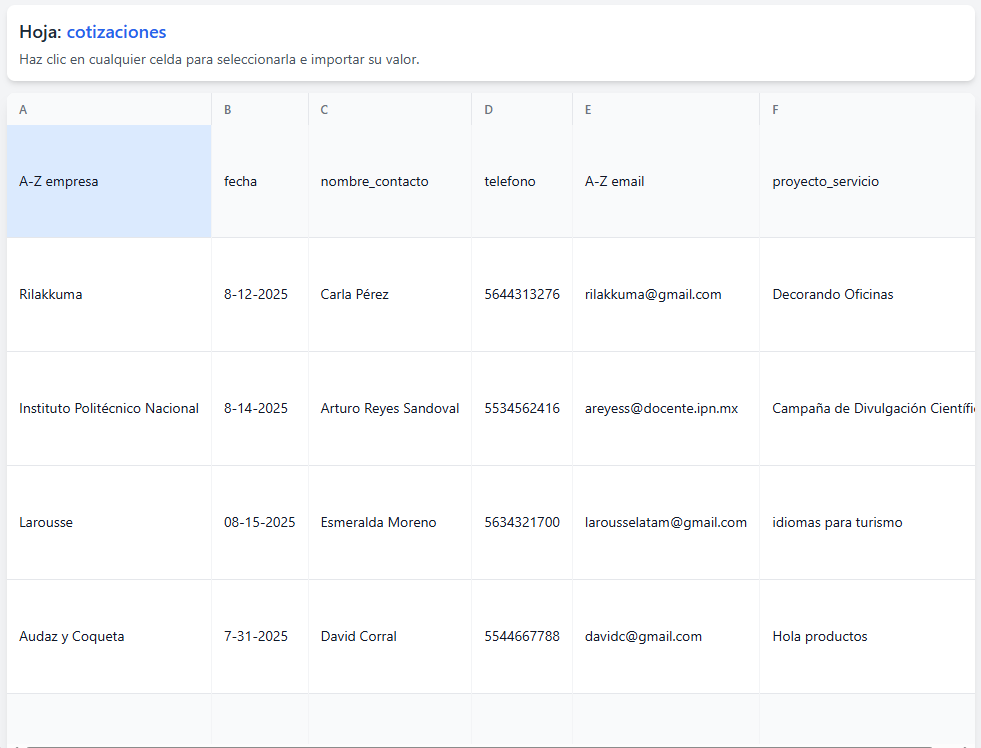
\includegraphics[width=0.8\textwidth]{Imagenes/ventana_importacion.png}
    \caption{Ventana de importación de datos}
    \label{fig:ventana_importacion}
\end{figure}


\subsubsection{Gestión de productos/servicios}

Para agregar productos, se incluyo una tabla, donde se pueden agregar, editar o eliminar productos o servicios con campos, con las mismas opciones de importación desde Excel.

\begin{figure}[H]
    \centering
    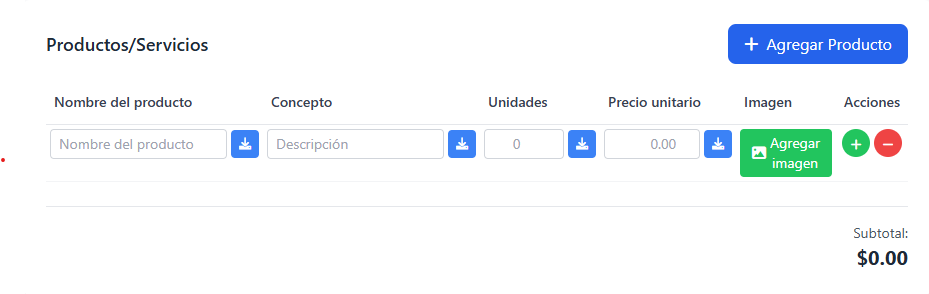
\includegraphics[width=0.8\textwidth]{Imagenes/tabla_productos.png}
    \caption{Tabla de productos/servicios}
    \label{fig:tabla_productos} 
\end{figure}

Una vez concluida la cotizacion y verificada la informacion, se puede guardar la cotizacion con el siguiente boton.

\begin{figure}[H]
    \centering
    
\includegraphics[width=0.8\textwidth]{Imagenes/boton_guardar.png}
    \caption{Botón para guardar la cotización}
    \label{fig:boton_guardar}
\end{figure}

\subsubsection{Opciones de guardado}

%%%%%%%%%%%%%%%%%%%%%%%%%%%%%%%%%%%%%%%%%%%%%%%%%%%%
\section{Ejemplos prácticos}
\subsection{Cómo registrar una cotización}
\subsection{Generación del PDF de la cotización}
\subsection{Ejemplo de cotización completa}
%%%%%%%%%%%%%%%%%%%%%%%%%%%%%%%%%%%%%%%%%%%%%%%%%%%%
\section{Resolución a problemas comunes}

\subsection{No abre correctamente el archivo excel}

En caso de que no abra correctamente el archivo excel, asegúrese de que el archivo esté en formato .xlsx y que la hoja seleccionada contenga datos válidos. Verifique también que el archivo no esté protegido con contraseña.

\subsection{Error al generar el PDF}

Asegurate de que todos los campos obligatorios esten completos y que haya errores en los datos ingresados. Si el problema persiste, intente reiniciar la aplicación y volver a generar el PDF.

\subsection{No se muestran las imágenes}

Asegúrese de que las imágenes estén en el formato correcto (JPEG, PNG) y que la ruta del archivo sea válida. Verifique también que las imágenes no estén dañadas.

\subsection{Problemas al ingresar datos}

Este puede ser un error comun en la aplicacion, en caso de que no se pueda ingresar algun campo, cambie a otra aplicacion y vuelva a la aplicacion de cotizaciones, esto deberia solucionar el problema.

\subsection{Soporte y contacto}

Para aistencia adicional, puedes contactar al soporte técnico a través del correo electrónico: aaronugaldet@gmail.com
\pagebreak

\end{document}